\documentclass[10pt,twocolumn]{article}
\usepackage[margin=0.72in]{geometry}
\usepackage{amsmath,amssymb,amsthm}
\usepackage{booktabs}
\usepackage{graphicx}
\usepackage{xcolor}
\usepackage{xurl}
\usepackage{hyperref}
\usepackage{microtype}

\hypersetup{
  colorlinks=true,
  linkcolor=blue!60!black,
  citecolor=blue!60!black,
  urlcolor=blue!60!black
}

\title{\textbf{Formal Algebraic, Combinatorial, and Rational-Enclosure Certification for Trifferent Codes}}
\author{Lluis Eriksson\\
\small Independent Researcher \quad $\cdot$ \quad \texttt{TRIFF-CERT-1.0}\\
\small \url{https://github.com/lluiseriksson/trifferent-codes-certificates}}
\date{November 26, 2026}

\begin{document}
\maketitle

\begin{abstract}
We present a machine-checked constructive Lean~4.35.0 kernel and zero-float exact rational certificate suite (\texttt{TRIFF-CERT-1.0}) auditing core algebraic, coding-theoretic, binary-box, and exact-logarithm pillars of Bhandari and Khetan's improved trifferent code bounds $T(n) = \Omega(1.162579^n)$ and $T(n) = O(n^{-1/2}(3/2)^n)$ (\texttt{arXiv:2611.33212v1}, Nov.\ 2026). Our artifact combines 18 constructive Lean~4.35.0 theorems (\texttt{0 sorry}, \texttt{0} custom axioms, \texttt{0 Classical.choice}, \texttt{0} warnings), an AST-audited zero-float Python verifier over $\mathbb{Z}$ and $\mathbb{Q}$, 16 canonical JSON certificates (\texttt{C01}--\texttt{C16}), and 37 unit and forgery-rejection tests. Inside Lean we prove the 9-word tetracode's constant Hamming distance~3 and rainbow-iff-distinct equivalence over $\mathbb{F}_3^4$, $\mathrm{AGL}(1,9)$ invertibility and injectivity (hence bijectivity) over $\mathbb{F}_3[i]/(i^2+1)$, the factorial cardinality formula $9\cdot 8\cdot (\mathrm{fact}\,14/(\mathrm{fact}\,4\cdot \mathrm{fact}\,3)) = 43{,}589{,}145{,}600$, $1.162579^4 > 9/5$, Appendix~A.2 port-cut identities, Section~3.6 inequalities $\binom{t}{3} \ge 3t-8$, ternary Tur\'{a}n, and $nD \le 96Z$, and Appendix~A.4's uniform logarithm-enclosure bound $1 - \chi^2 \ge 8/9$. In Python we independently verify $\mathrm{AGL}(1,9)$ sharp 2-transitivity, exact pair counts $H_0,\dots,H_{14}$ via binomial inversion, first-principles Lemma~3.2 central-hole contradiction across all 48 sign configurations on Eq.~(25), exact $3^n$ binary-box counts on finite trifferent codes through $n=5$, and Appendix~A.4 exact rational logarithm enclosures certifying $\bar{N} > 1.162579^n$ at blocklengths $n = 124k$ ($k \ge 1$).
\end{abstract}

\section{Introduction and Audited Scope}

A ternary code $C \subseteq \mathbb{F}_3^n$ is \emph{trifferent} if every three distinct codewords $x, y, z \in C$ admit a \emph{rainbow coordinate} $i \in [n]$ with $\{x_i, y_i, z_i\} = \{0, 1, 2\}$. Let $T(n)$ denote the maximum size of a trifferent code of blocklength $n$. Bhandari and Khetan~\cite{bhandari2026triff} improve both sides of this extremal problem:
\begin{equation}
  T(n) = \Omega(1.162579^n), \qquad T(n) = O\!\left(n^{-1/2}(3/2)^n\right).
\end{equation}
Their lower bound beats the 1988 K\"{o}rner--Marton base $(9/5)^{1/4} \approx 1.158292$~\cite{korner1988} and Yuan--Zhu's $1.158344$~\cite{yuan2026} by encoding a random overlapping system of arity-$\ell=14$ local constraints $Q = \{x \in \mathbb{F}_9^{14} : \text{multiplicities } (4,3,1^7)\}$ through the 9-word tetracode $\psi(a,b) = (a, b, a+b, a-b) \in \mathbb{F}_3^4$ with independent uniform $\mathrm{AGL}(1,9)$ port permutations and two-stage alteration (deleting close pairs before far bad triples). Their upper bound improves $O(n^{-2/5}(3/2)^n)$ by establishing a central-hole coherence constraint (Lemma~3.2) among binary boxes avoiding masks $q \in \mathbb{F}_3^n$, yielding $D \le (96/n) Z \le (96/n) 3^n$ where $D$ counts double boxes ($f(q)=2$) and $Z$ counts empty boxes (holes, $f(q)=0$).

This work delivers an independent machine-checked audit (\texttt{TRIFF-CERT-1.0}) with an explicit scope boundary:
\begin{enumerate}
  \item \textbf{Constructive Lean~4.35.0 kernel} (\path{lean/TrifferentCodesCert.lean}): 18 constructive theorems (\texttt{0 sorry}, \texttt{0 Classical.choice}, audited via \texttt{\#print axioms}) formalizing the finite-field coding properties of $\psi$ and $\mathrm{AGL}(1,9)$ directly over \texttt{Fin 3}, exact integer base/cardinality identities, Appendix~A.2 port-profile cuts, Section~3.6 algebraic inequalities, and Appendix~A.4's denominator bound.
  \item \textbf{AST-audited zero-float verifier} (\path{src/trifferent_verifier.py}): performs four exact integer/rational verification modes over $\mathbb{Z}$ and $\mathbb{Q}$. We note honestly that we do \emph{not} replay the 11,713-leaf external triple-subdivision file of Appendix~A.3; rather, we audit the underlying local rule $Q$, exact pair-count table $H_0,\dots,H_{14}$, safe cuts Eqs.~(41)--(42), exact rational $\ln$ enclosures for $\bar{N} > g^n$, Lemma~3.2's finite contradiction table, and exact $3^n$ binary-box geometry on finite codes.
\end{enumerate}

\section{Constructive Lean 4.35.0 Kernel}

All 18 theorems in \texttt{TrifferentCodesCert.lean} build cleanly under Lean~4.35.0 with zero warnings and depend exclusively on at most \texttt{propext} and \texttt{Quot.sound} (zero \texttt{Classical.choice}). Theorems~1--4 formalize real finite-field coding-theoretic properties directly over \texttt{Fin 3}: constant Hamming distance~3 between all distinct tetracode words, the exact rainbow-iff-distinct equivalence on all $9^3 = 729$ triples, non-vanishing determinant $a'^2 + a''^2 \not\equiv 0 \pmod{3}$ for nonzero scalars in $\mathbb{F}_3[i]/(i^2+1)$, and injectivity (hence bijectivity) of every $\mathrm{AGL}(1,9)$ map on $\mathbb{F}_3^2$. Table~\ref{tab:lean} records all 18 quantified Lean statements in abbreviated mathematical syntax.

\begin{table*}[t]
\centering
\caption{Summary of all 18 constructive theorems in \texttt{TrifferentCodesCert.lean} (Lean~4.35.0, \texttt{0 sorry}, \texttt{0 Classical.choice}, \texttt{0} warnings).}
\label{tab:lean}
\footnotesize
\begin{tabular}{@{}rll@{}}
\toprule
\# & Lean Theorem Name & Exact Quantified Lean Statement (abbreviated syntax) \\
\midrule
1 & \texttt{tetracode\_constant\_distance\_3} & $\forall (a_1,b_1) \ne (a_2,b_2) \in \mathbb{F}_3^2,\; d_H(\psi(a_1,b_1), \psi(a_2,b_2)) = 3$ (0 axioms) \\
2 & \texttt{tetracode\_rainbow\_iff\_distinct} & $\forall (a_i,b_i) \in \mathbb{F}_3^2,\; \mathrm{hasRainbow}_4(\psi_1,\psi_2,\psi_3) = \text{pairwiseDistinct}$ \\
3 & \texttt{agl19\_invertible\_det\_nonzero} & $\forall (a',a'') \ne (0,0) \in \mathbb{F}_3^2,\; (a'^2 + a''^2) \bmod 3 \ne 0$ \\
4 & \texttt{agl19\_bijective\_on\_f9} & $\forall (a',a'') \ne (0,0),\, \mathrm{aglApply}(a',a'',b',b'',\cdot)$ is injective on $\mathbb{F}_3^2$ \\
5 & \texttt{local\_rule\_cardinality\_exact} & $9 \cdot 8 \cdot (\mathrm{fact}\,14 / (\mathrm{fact}\,4 \cdot \mathrm{fact}\,3)) = 43{,}589{,}145{,}600$ (0 axioms) \\
6 & \texttt{base\_beats\_korner\_marton\_and\_yuan\_zhu} & $9 \cdot 10^{24} < 5 \cdot 1162579^4 \land 1158344 < 1162579$ (0 axioms) \\
7 & \texttt{wiring\_degree\_port\_balance} & $\forall k,\; 9k+22k=31k \land 2(9k)+3(22k)=84k \land 6k\cdot 14=84k \land 4(31k)=124k$ \\
8 & \texttt{min\_distance\_nine\_thirty\_seconds} & $\forall m,\; 32(9m) = 9 \cdot 8(4m)$ (certifying $3\delta m = 9n/32$ at $\delta=3/8$) \\
9 & \texttt{equality\_state\_probability\_sums} & $1+8=9 \land 1+8+8+8=25 \land 25+56=81$ (0 axioms) \\
10 & \texttt{port\_cut\_pair\_state\_69\_224} & $\forall k,\; 224(9(31k) - 8(9k)) = 69 \cdot 8(84k)$ (Eq.~41: $h_i + h_{i'} \ge 69/224$) \\
11 & \texttt{port\_cut\_all\_equal\_31\_64} & $\forall k,\; 64(27(31k) - 16(9k)) = 33 \cdot 16(84k) \land 33+31=64$ ($h_A \le 31/64$) \\
12 & \texttt{port\_cuts\_31\_56\_and\_93\_224} & $\forall k,\; 56(12(31k)) = 31 \cdot 8(84k) \land 224(9(31k)) = 93 \cdot 8(84k)$ (Eqs.~41--42) \\
13 & \texttt{binomial\_cubic\_lower\_bound} & $\forall t \in \mathbb{N},\; 6(3t) \le t(t-1)(t-2) + 48$ ($\binom{t}{3} \ge 3t - 8$) \\
14 & \texttt{contact\_to\_hole\_ratio\_16\_3} & $\forall H,A,Z,\; 3A \le 3H + 8Z \to 2H \le A \to 3A \le 16Z$ \\
15 & \texttt{ternary\_turan\_pair\_diff} & $\forall m_0,m_1,m_2 \in \mathbb{Z},\; 3(m_0 m_1 + m_0 m_2 + m_1 m_2) \le (m_0+m_1+m_2)^2$ \\
16 & \texttt{double\_box\_density\_96} & $\forall M \ge 4,\, 3A \le 16Z,\, n(M-3)D \le 6(M-1)A \to nD \le 96Z$ (Eq.~37) \\
17 & \texttt{quadratic\_root\_subadditive} & $\forall b, s \in \mathbb{N},\; b^2 + s^2 \le (b+s)^2$ \\
18 & \texttt{log\_enclosure\_denominator\_bound} & $\forall p, q \in \mathbb{N},\; 3p \le q \to 8q^2 \le 9(q^2 - p^2)$ ($1-\chi^2 \ge 8/9$) \\
\bottomrule
\end{tabular}
\end{table*}

\section{Zero-Float Exact Rational Verification Modes}
\label{sec:modes}

The Python verifier \path{src/trifferent_verifier.py} is statically AST-audited by \texttt{pytest} for zero floating-point operations (strictly \texttt{int} and \texttt{fractions.Fraction}, rejecting \texttt{bool}-as-\texttt{int} and unreduced fractions).

\paragraph{Mode 1 (\texttt{tetracode\_and\_agl19}, \texttt{C01}).}
Constructs the 9-word tetracode $\psi(\mathbb{F}_3^2) \subset \mathbb{F}_3^4$, checks constant distance~3 on all $\binom{9}{2}=36$ pairs and rainbow coordinates on all $\binom{9}{3}=84$ triples, enumerates all 72 affine maps $\mathrm{AGL}(1,9)$ over $\mathbb{F}_3[i]/(i^2+1)$, confirms every map is bijective with nonzero determinant, and verifies sharp 2-transitivity (every ordered distinct pair of $\mathbb{F}_9$ is attained uniquely as $(f(0,0), f(1,0))$).

\paragraph{Mode 2 (\texttt{local\_rule\_counts}, \texttt{C02}).}
Computes $|Q| = 43{,}589{,}145{,}600$ and the exact pair-agreement counts $H_0,\dots,H_{14}$ of Appendix~A.1 of~\cite{bhandari2026triff} via exact rational polynomial multiplication over all 72 rearrangements of $(4,3,1^7)$ followed by binomial inversion $H_i = \sum_{j=i}^{14} (-1)^{j-i} \binom{j}{i} \Delta_j$. This yields $H_0 = 8{,}384{,}898{,}759$, $H_1 = 14{,}669{,}424{,}451$, $H_{14} = 1$, $\sum_{j=0}^{14} H_j = |Q|$, and exact mean agreement $\mathbb{E}[J] = \sum_j j H_j / |Q| = 14/9$ (Fig.~\ref{fig:pair}).

\begin{figure}[t]
  \centering
  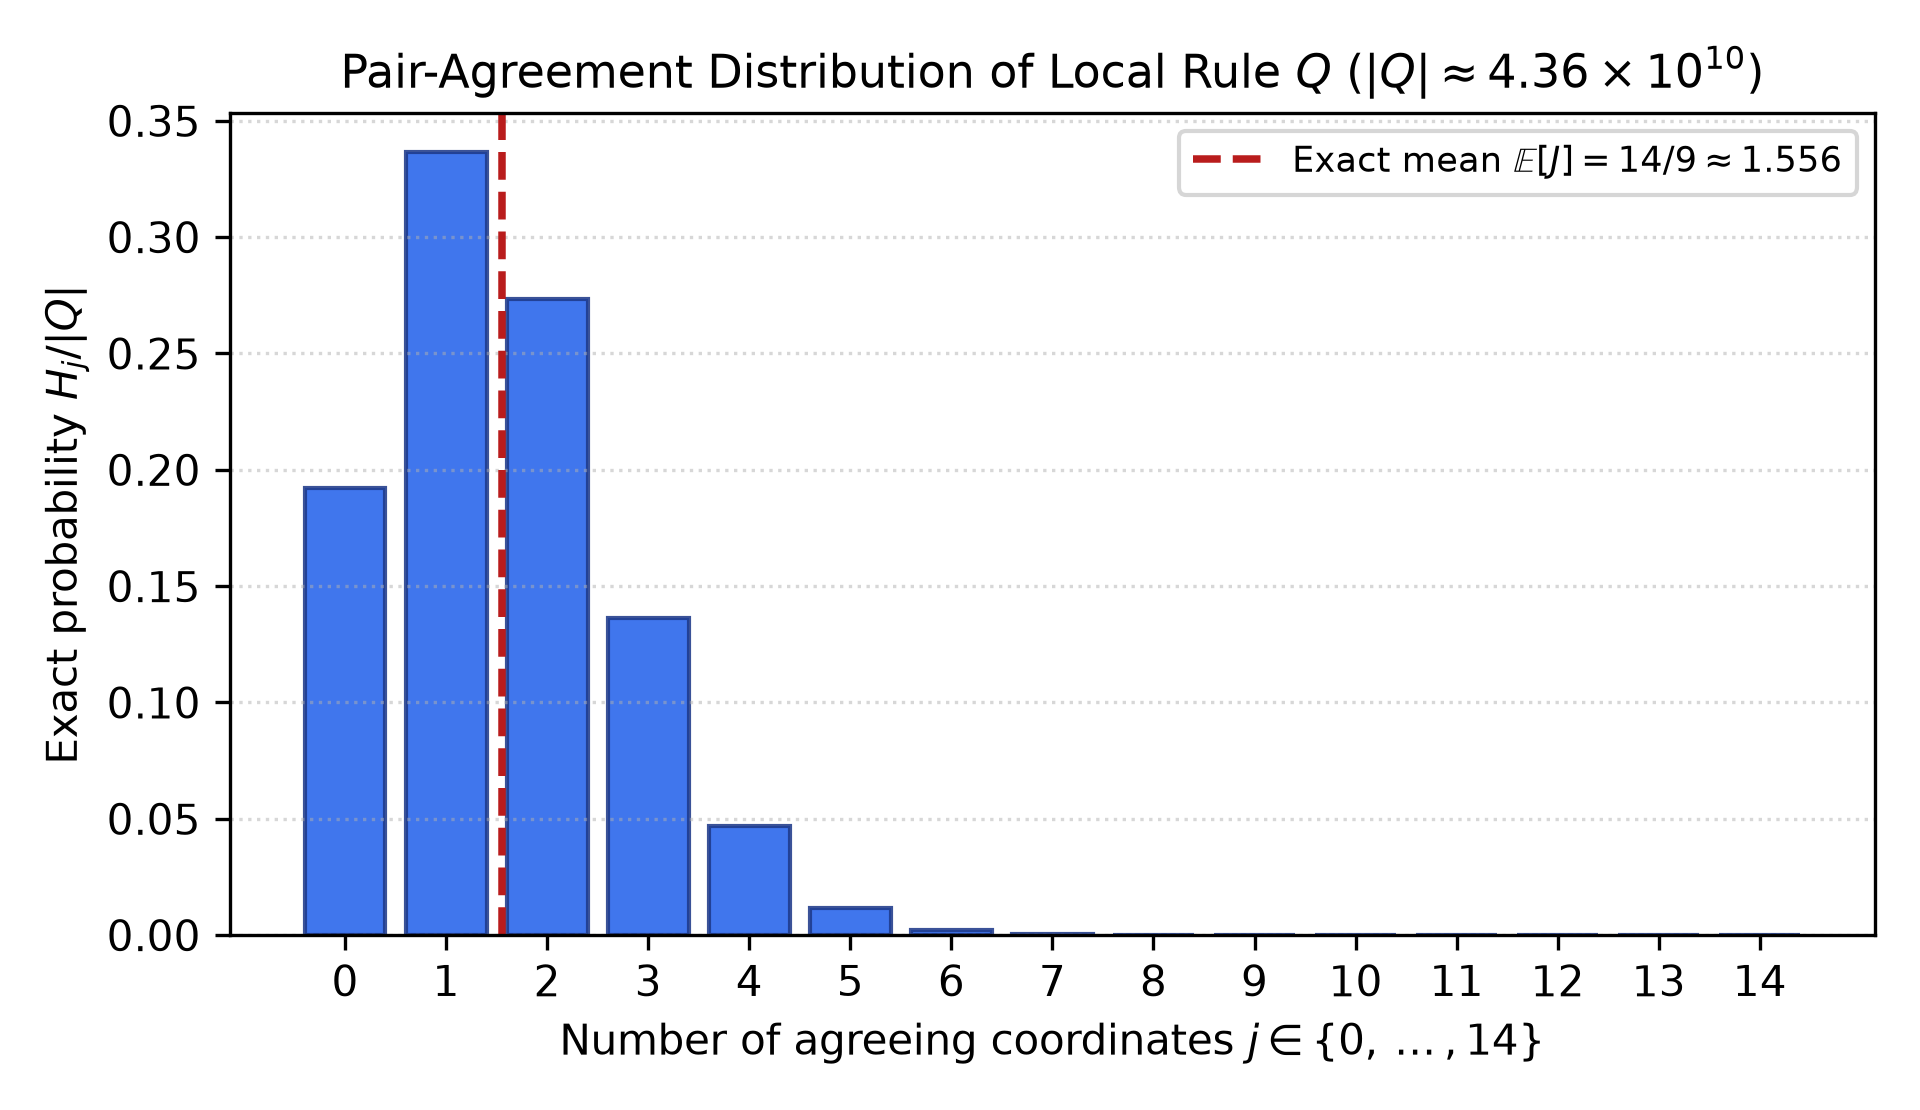
\includegraphics[width=\linewidth]{figures/fig1_local_rule_pair_distribution.png}
  \caption{Exact pair-agreement probability distribution $H_j/|Q|$ ($j=0,\dots,14$) computed via Appendix~A.1 binomial inversion over $\mathbb{Q}$, confirming exact mean $\mathbb{E}[J] = 14/9$.}
  \label{fig:pair}
\end{figure}

\paragraph{Mode 3 (\texttt{section3\_upper\_bound}, \texttt{C03}--\texttt{C08}).}
Audits explicit finite trifferent codes for $n \in \{2,3,4,5\}$ by exhaustive triple verification and full $3^n$ binary-box enumeration, computing double boxes $D$, holes $Z$, and hole-contact degree sum $A = \sum_{f(q)=0} d_q$, verifying exact pair-count identities Eqs.~(35)--(36) ($D = \sum_{\{x,y\}} 2^{n-d(x,y)}$ and $2A = \sum_{\{x,y\}} (n-d(x,y)) 2^{n-d(x,y)}$) and the Section~3.6 bounds $3A \le 16Z$ and $nD \le 96Z$ (e.g., on the optimal $n=4, M=9$ tetracode in \texttt{C05}: $D=72, Z=9, A=36$, giving $3A=108 \le 144=16Z$ and $nD=288 \le 864=96Z$). Additionally, for \texttt{C03}--\texttt{C05}, Mode~3 verifies Lemma~3.2 from first principles on the Eq.~(25) core ($A_0{=}000, A_1{=}111, A_2{=}222, B_0{=}012, B_1{=}120, B_2{=}201$): checking core trifference, confirming $h{=}021$ and $h'{=}102$ are valid single-agreement hole masks, deriving contact pairs and $f(B), g(B)$ directly from the masks, deriving $X{=}110, Y{=}202$ and each $(Z,T)$ pair by filtering the 8 hole-avoiding prefixes against the same-sign rainbow condition, and exhausting all 48 sign assignments $(r,x,y,z,t) \in \{0,1,2\}\times\{-1,+1\}^4$ against Eq.~(32).

\paragraph{Mode 4 (\texttt{log\_enclosures\_and\_port\_cuts}, \texttt{C09}--\texttt{C16}).}
Implements Appendix~A.4's exact rational logarithm enclosure $\xi = 2^p y$ ($1 \le y < 2$), $\chi = (y-1)/(y+1) \in [0, 1/3]$,
\begin{equation}
  L_q(\chi) \le \ln y \le L_q(\chi) + \frac{2\chi^{2q+1}}{(2q+1)(1-\chi^2)},
\end{equation}
entirely over $\mathbb{Q}$ (zero floats), certifies $g^4 > 9/5$ (Fig.~\ref{fig:base}), verifies the Appendix~A.2 safe port-profile cuts $(69/224, 31/64, 31/56, 93/224)$, and certifies Eq.~(9)'s expected-codeword inequality $\bar{N}^{1/k} = 9^{31}(|Q|/9^{14})^6 > g^{124}$ via $6\,\mathrm{lo}(\ln|Q|) - 53\,\mathrm{hi}(\ln 9) > 124\,\mathrm{hi}(\ln g)$ at $g = 1162579/1000000$ across series orders $q \in \{8, 10, 20, 40, 60\}$ (Fig.~\ref{fig:log}).

\begin{figure}[t]
  \centering
  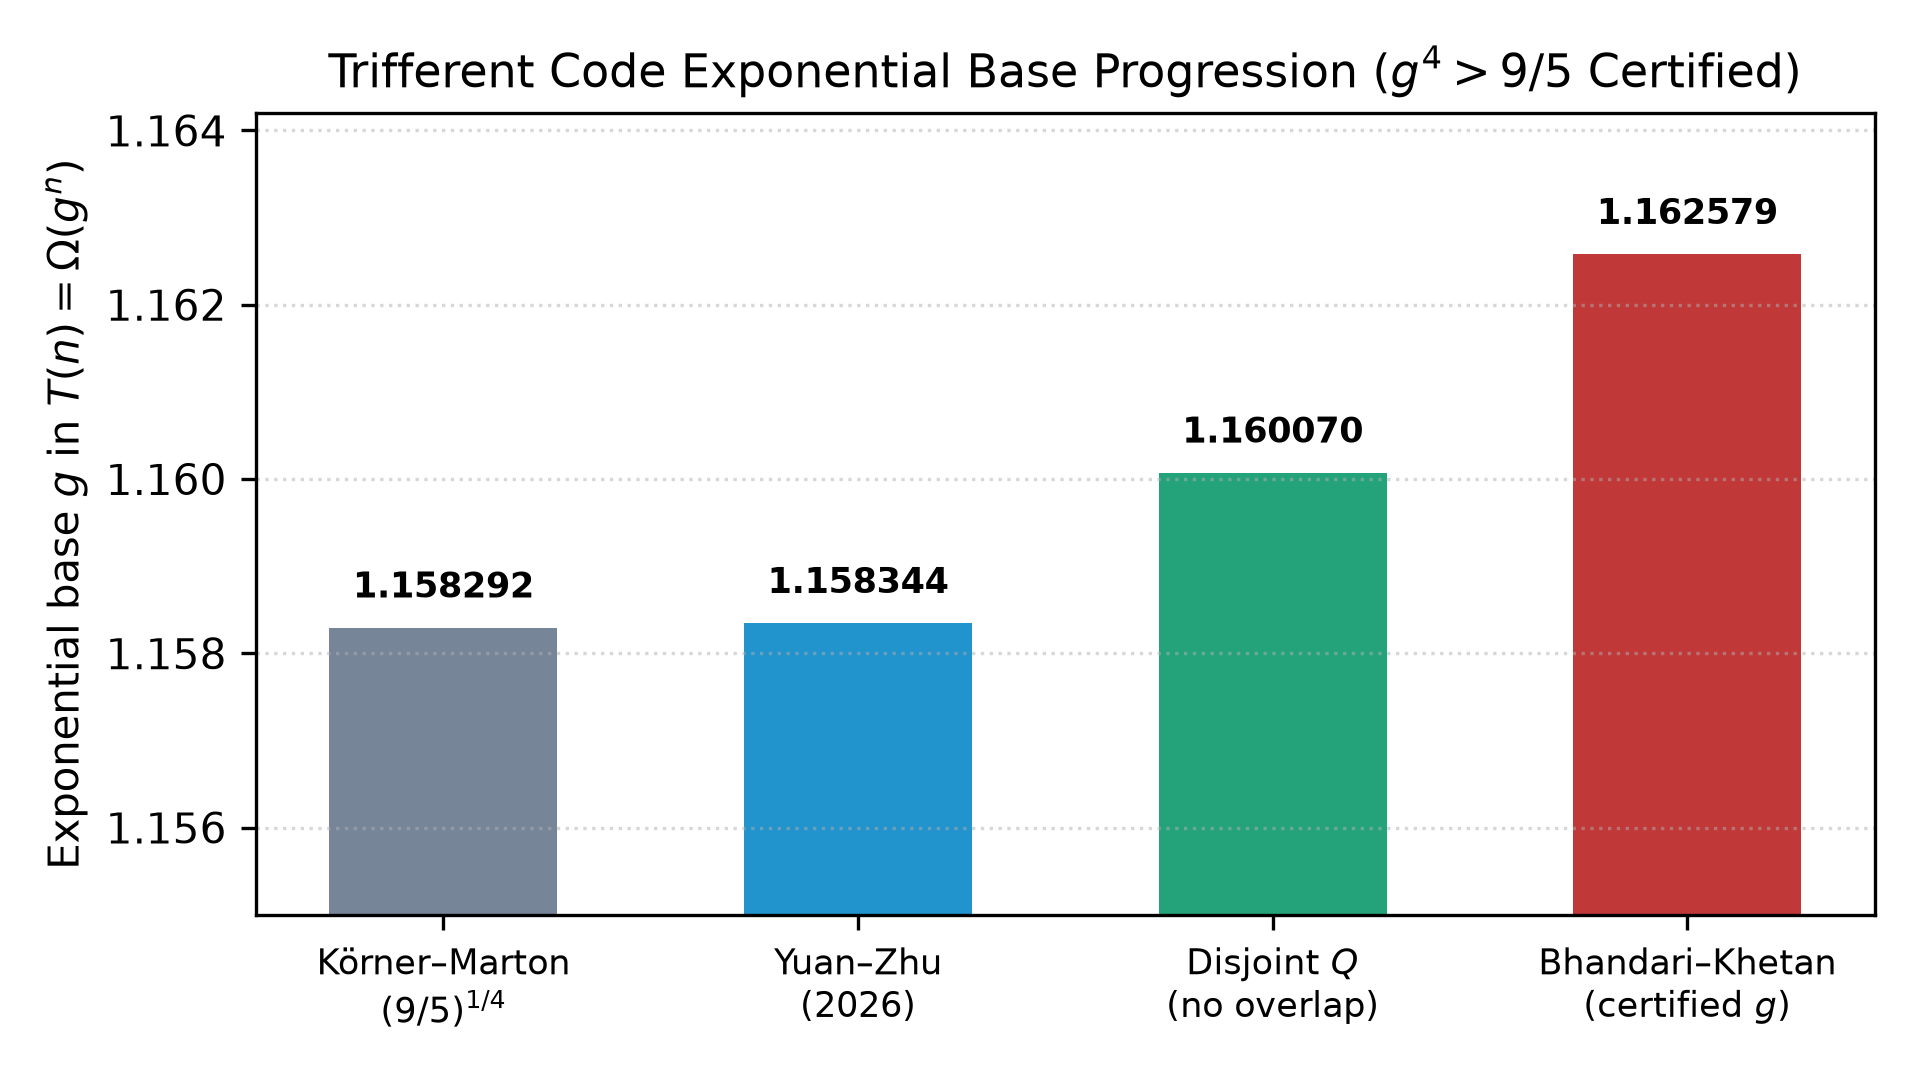
\includegraphics[width=\linewidth]{figures/fig2_exponential_base_progression.png}
  \caption{Progression of trifferent-code exponential lower-bound bases from K\"{o}rner--Marton $(9/5)^{1/4}$ and Yuan--Zhu~\cite{yuan2026} through disjoint-$Q$ blocks to Bhandari--Khetan's overlapping-constraint base $g = 1.162579$.}
  \label{fig:base}
\end{figure}

\begin{figure}[t]
  \centering
  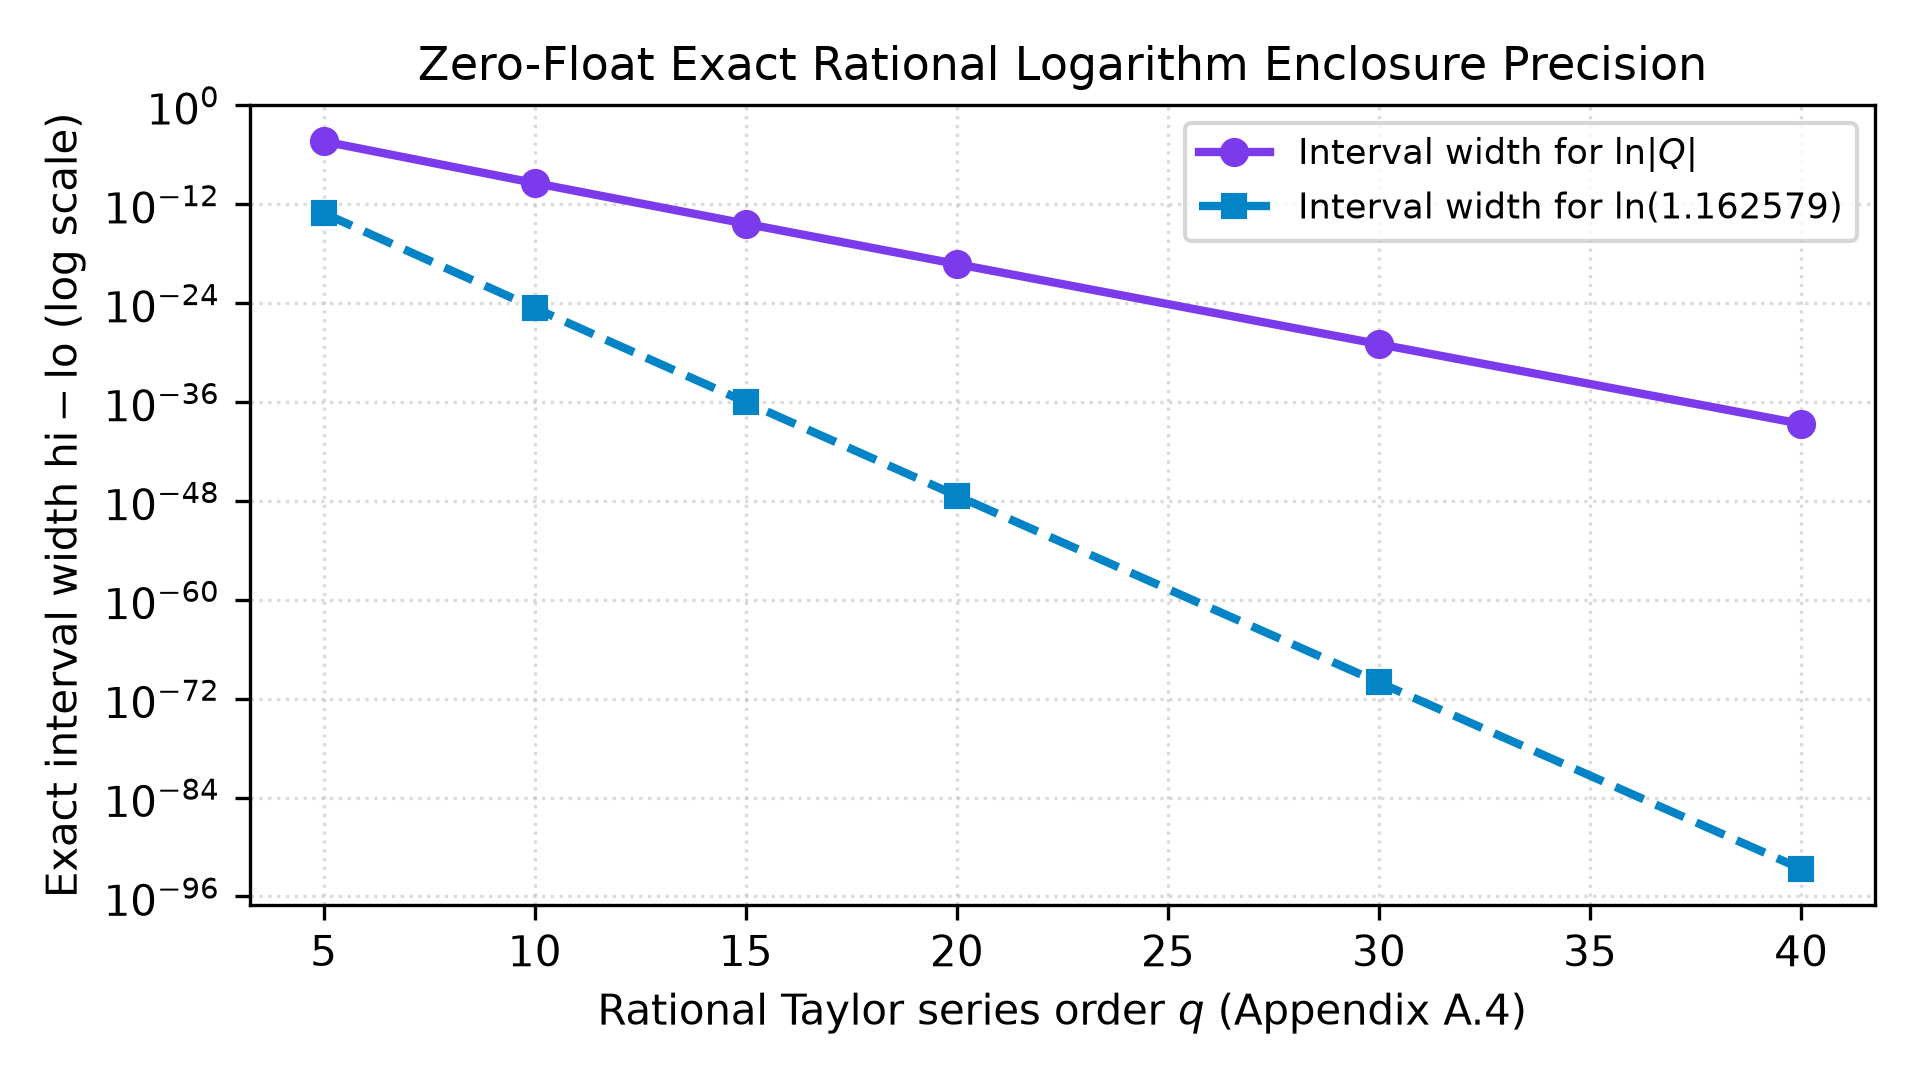
\includegraphics[width=\linewidth]{figures/fig3_log_enclosure_precision.png}
  \caption{Exact rational logarithm enclosure interval width $\mathrm{hi}-\mathrm{lo}$ for $\ln |Q|$ and $\ln(1.162579)$ versus Appendix~A.4 series order $q$, shrinking below $10^{-38}$ ($2.19 \times 10^{-39}$) and $10^{-92}$ ($2.28 \times 10^{-93}$) by $q=40$.}
  \label{fig:log}
\end{figure}

\section{Certificate Suite and Adversarial Testing}

Table~\ref{tab:certs} summarizes all 16 canonical certificates (\texttt{C01}--\texttt{C16}). Our test suite (\path{tests/test_verifier.py}) executes 37 tests in under $0.3\text{ s}$: all 16 certificates, the AST zero-float audit, and 20 adversarial forgery/type tests covering schema/mode tampering, forged tetracode distance and $\mathrm{AGL}(1,9)$ order, altered $|Q|$ and $H_0$, non-trifferent/duplicate/invalid-symbol codes, forged $D$ and $Z$, bases below $(9/5)^{1/4}$ or exceeding $\bar{N}^{1/n}$, disabled \texttt{verify\_Nbar\_ge\_gn}, forged Appendix~A.2 port cuts, non-\texttt{Fraction} log input, unreduced fractions, float/\texttt{bool} coercion, and invalid $n/k$.

\begin{table}[t]
\centering
\caption{Canonical certificate inventory (\texttt{TRIFF-CERT-1.0}, 16/16 verified over $\mathbb{Q}$).}
\label{tab:certs}
\scriptsize
\setlength{\tabcolsep}{1.2pt}
\begin{tabular}{@{}llll@{}}
\toprule
ID & Mode & Witness / Params & Exact Certified Output \\
\midrule
C01 & 1 & Tetra + $\mathrm{AGL}(1,9)$ & $M{=}9, d{=}3, 84$ tr., $|\mathrm{AGL}|{=}72$ \\
C02 & 2 & Rule $Q$ ($4,3,1^7$) & $|Q|{=}43589145600$, $\mathbb{E}[J]{=}14/9$ \\
C03 & 3 & $n{=}2, M{=}4$ + L3.2 & $D{=}8, Z{=}1, A{=}2$; 48/48 contra. \\
C04 & 3 & $n{=}3, M{=}6$ + L3.2 & $D{=}24, Z{=}3, A{=}9$; 48/48 contra. \\
C05 & 3 & Tetra $n{=}4, M{=}9$ & $D{=}72, Z{=}9, A{=}36$; $nD{\le}96Z$ \\
C06 & 3 & Subcode $n{=}4, M{=}6$ & $D{=}30, Z{=}15, A{=}15$; $3A{\le}16Z$ \\
C07 & 3 & Boundary $n{=}3, M{=}4$ & $D{=}9, Z{=}4, A{=}3$; $nD{\le}96Z$ \\
C08 & 3 & Lifted $n{=}5, M{=}9$ & $D{=}144, Z{=}99, A{=}144$ ($3^5$ box) \\
C09 & 4 & $g{=}1.162579$, $q{=}10$ & $\bar{N}{>}g^n$ \& Eq.~(41)--(42) cuts \\
C10 & 4 & $g{=}1.162579$, $q{=}20$ & $\bar{N}{>}g^n$ (exact $\mathbb{Q}$ enclosure) \\
C11 & 4 & $g{=}1.162579$, $q{=}40$ & $\bar{N}{>}g^n$ (width $<10^{-38}$) \\
C12 & 4 & $g{=}29/25{=}1.16, q{=}12$ & Beats $(9/5)^{1/4}$, $\bar{N}{>}g^n$ \\
C13 & 4 & Yuan--Zhu $1.158344$ & Beats $(9/5)^{1/4}$, $\bar{N}{>}g^n$ \\
C14 & 4 & Disjoint $Q$ $1.16007$ & Beats $(9/5)^{1/4}$, $\bar{N}{>}g^n$ \\
C15 & 4 & $g{=}1.162579$, $q{=}8$ & Cuts $(69/224,31/64,31/56,93/224)$ \\
C16 & 4 & $g{=}1.162579$, $q{=}60$ & Ultra-tight $\bar{N}{>}g^n$ enclosure \\
\bottomrule
\end{tabular}
\end{table}

\section{Reproducibility and Disclosure}

All files are SHA-256 hashed in \texttt{MANIFEST.sha256} and archived at \url{https://github.com/lluiseriksson/trifferent-codes-certificates} (\texttt{v1.0.0}). Independent reproduction requires only Lean~4.35.0 and Python~3.10+:
\begin{quote}\raggedright\footnotesize\ttfamily
cd lean \&\& lake build \&\& cd ..\\
python scripts/generate\_certificates.py\\
python -m src.trifferent\_verifier certificates/\\
pytest -q
\end{quote}
\noindent\textbf{AI-Assisted Formalization Disclosure.} This verification artifact was authored by Lluis Eriksson using Google Antigravity for Lean~4 proof engineering, zero-float Python verification scripting, test design, and manuscript preparation. Every verified claim is scoped strictly to the 18 Lean~4.35.0 theorems and 16 exact-rational certificates (\texttt{C01}--\texttt{C16}).

\begin{thebibliography}{3}
\bibitem{bhandari2026triff}
S.~Bhandari and A.~Khetan,
\emph{Constructions and Upper Bounds for Trifferent Codes},
arXiv:2611.33212v1, November 2026.
\bibitem{korner1988}
J.~K\"{o}rner and K.~Marton,
\emph{New bounds for perfect hashing via information theory},
European J.\ Combin.\ \textbf{9} (1988), 523--530.
\bibitem{yuan2026}
C.~Yuan and R.~Zhu,
\emph{Beating the probabilistic bound for hashing and improving lower bounds for trifferent codes},
arXiv:2611.11262, 2026.
\end{thebibliography}

\end{document}
